%! Author = vanchondo
%! Date = 10/06/2020

\section{Methodology}

La metodología utilizada es CRISP-DM.\@
\begin{enumerate}
      \item Comprensión del negocio (Business Understanding). \\Los objetivos de este
            proyecto son:
            \begin{itemize}
                  \item Poder reconocer e interpretar las expresiones faciales de un grupo de personas
                        durante la presentación de un discurso, comercial o producto nuevo.
                  \item Una vez procesada la información, poder entregar al cliente un
            \end{itemize}

      \item Comprensión de datos (Data Understanding) Para poder comprender e interpretar
            la información recolectada, se diseñará un clasificador el cual será entrenado
            utilizando un data set existente llamado
            AffectNet\cite[]{mollahosseini2017affectnet}, el cual cuenta con las siguientes
            clasificaciones:
            \begin{table}[h!]
                  \centering
                  \caption{
                  Número de imagenes clasificadas en cada categoría.
                  {
                  \label{tab:stats_num_data}
                  \cite[]{mollahosseini2017affectnet}
                  }
                  }
                  \begin{tabular}{ |c|c| }
  \hline
  \toprule
  Expression & Number  \\
  \midrule
  Neutral    & 80,276  \\
  Happy      & 146,198 \\
  Sad        & 29,487  \\
  Surprise   & 16,288  \\
  Fear       & 8,191   \\
  Disgust    & 5,264   \\
  Anger      & 28,130  \\
  Contempt   & 5,135   \\
  None       & 35,322  \\
  Uncertain  & 13,163  \\
  Non-Face   & 88,895  \\
  \bottomrule
  \hline
\end{tabular}
            \end{table}
      \item Preparación de datos (Data Preparation). \\Para preparar los datos se realizan
            los siguientes pasos:
            \begin{itemize}
                  \item La información será capturada con una o mas cámaras las cuales tomaran fotos al
                        grupo muestra de personas durante la presentación.
                  \item Se procesan las fotos para separar los rostros detectados en una foto en
                        imágenes diferentes.
                        \begin{figure}[h]
                              \centering
                              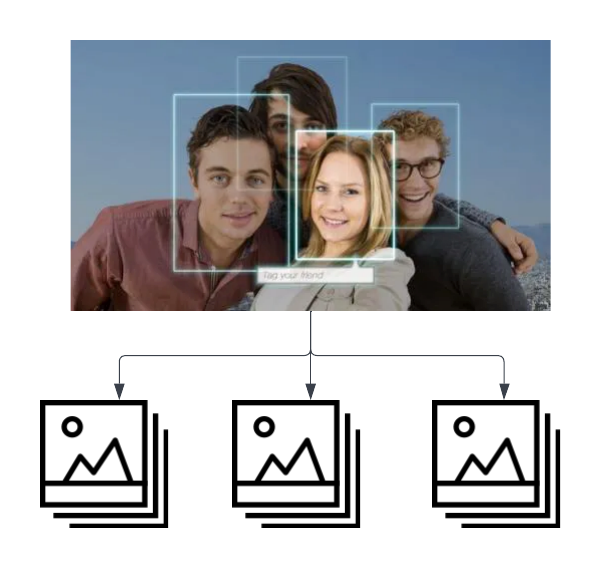
\includegraphics[width=8cm]{figures/pictureSplit.png}
                              \caption{Imagen ilustrativa de la detección y separación de los rostros en multiples imagenes.}
                              \caption*{Source: https://computerhoy.com/noticias/life/reconocimiento-facial-ventajas-peligros-revolucion-69441}
                        \end{figure}

                  \item Se aplican técnicas de limpieza sobre la imagen para eliminar la existencia de
                        ruido.
            \end{itemize}

      \item Modelado (Modeling) \\Las imágenes se categorizan por lapsos de tiempo, por
            ejemplo, cada 5 segundos, este tiempo es personalizable, para así poder obtener
            los cambios de los rostros faciales del publico de una manera promediada y
            saber mejor el impacto que se esta obteniendo debido a la presentación.

      \item Evaluación (Evaluation) \\Para la evaluación, se van a ejecutar múltiples
            experimentos con grupos de personas diversos, por ejemplo, un grupo de
            estudiantes de primaria, secundaria y prepa en donde se les presente el tráiler
            de una nueva película. \\Al finalizar, se realiza una encuesta para obtener
            información básica sobre que fue lo que sintieron durante la presentación. \\De
            esta forma podremos verificar si los resultados obtenidos por el sistema son
            similares al obtenido de la encuesta. \\Algo a tener en mente es que para las
            personas es mas fácil quedarse con el sentimiento de lo ultimo que vieron,
            entonces si el inicio de la presentación les pareció muy interesante y el final
            muy aburrido, podríamos llegar a obtener resultados diferentes, dicho esto, se
            recomienda que para las evaluaciones se utilicen presentaciones de periodos
            cortos y que no abusen de las emociones del publico.

      \item Implementación (Deployment) \\Para la implementación se planea hacer uso de
            servicios en la nube para realizar todo el procesamiento de la información. \\Y
            el uso de un equipo moderado para la captura de las imágenes tales como cámaras
            y una computadora para poder subir esta información a nuestro servicio para
            iniciar el procesamiento.
            \begin{figure}[h]
                  \centering
                  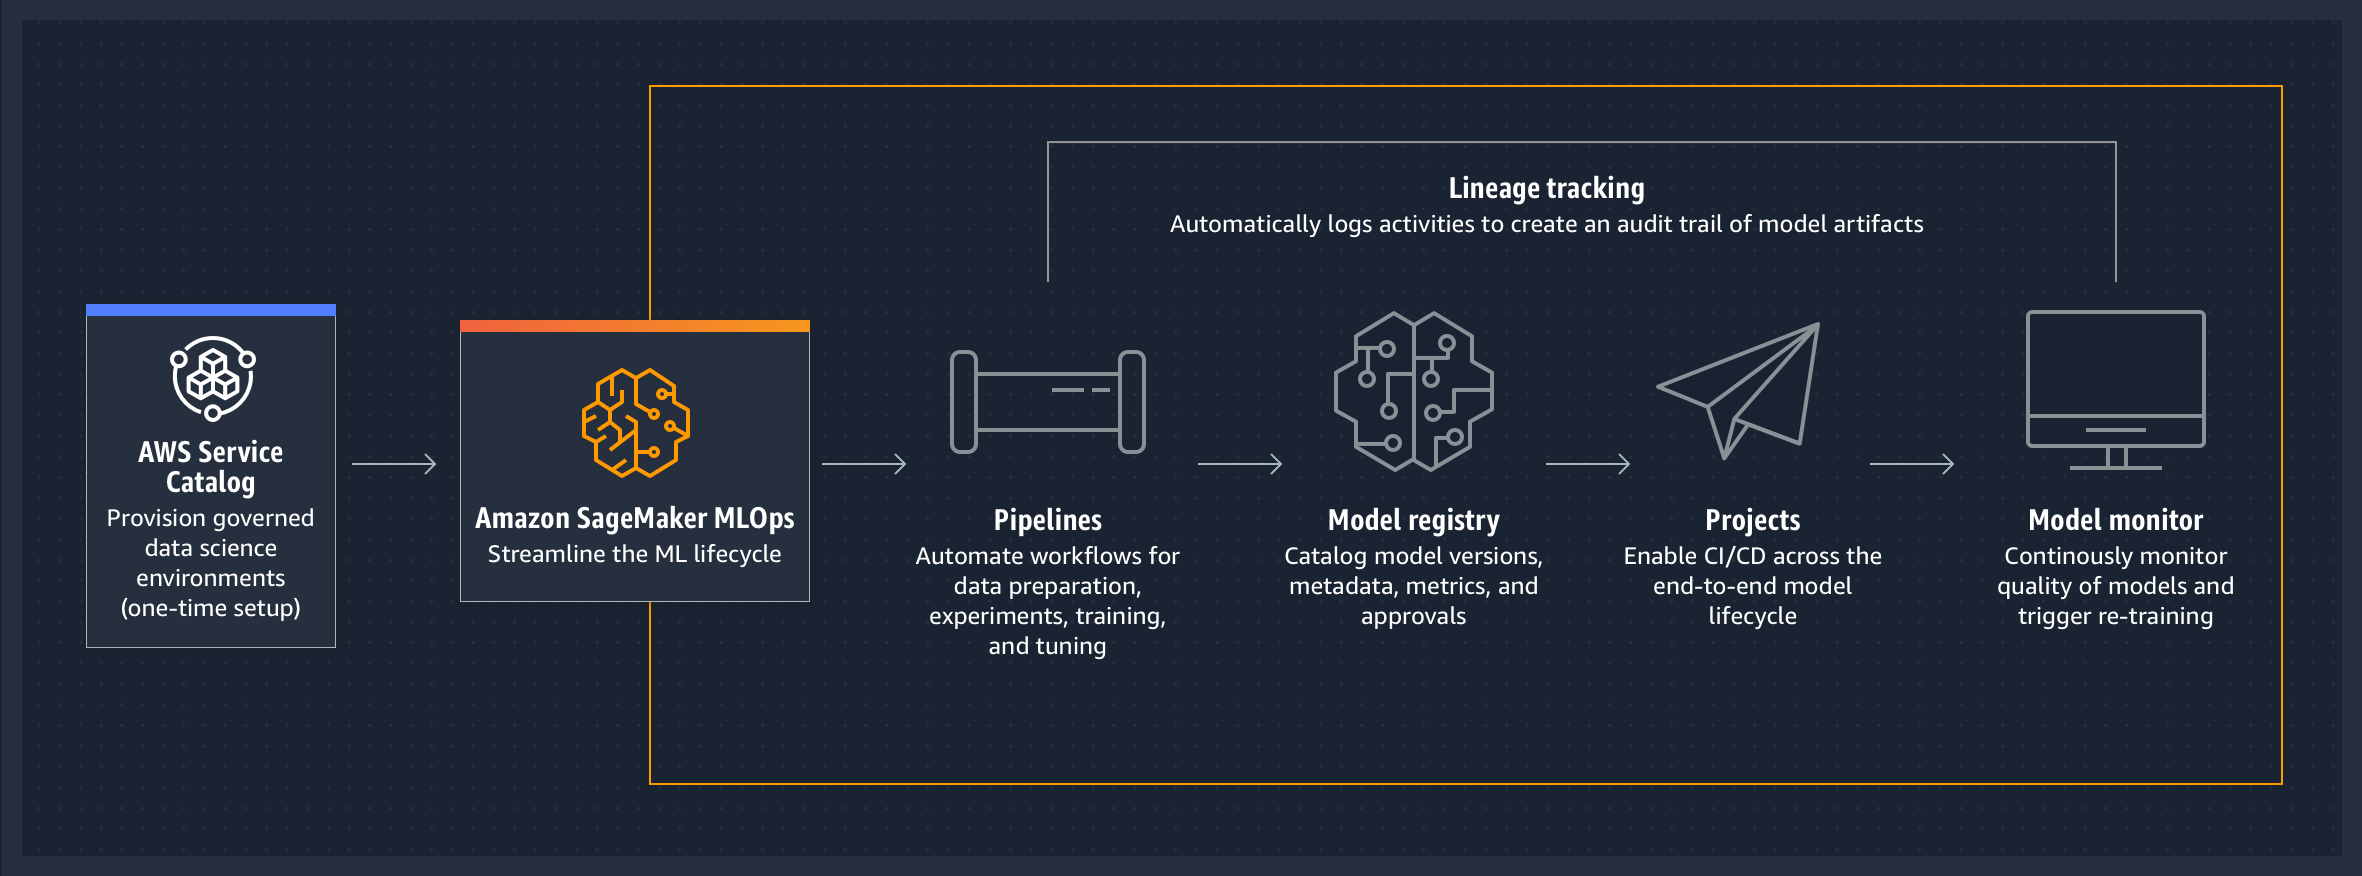
\includegraphics[width=9cm]{figures/sageMakerAWS.png}
                  \caption{Amazon SageMaker}
                  \caption*{Source: https://aws.amazon.com/sagemaker/mlops/}
            \end{figure}
\end{enumerate}